\documentclass{standalone}
\usepackage{tikz}
\usetikzlibrary{patterns, positioning}


\begin{document}
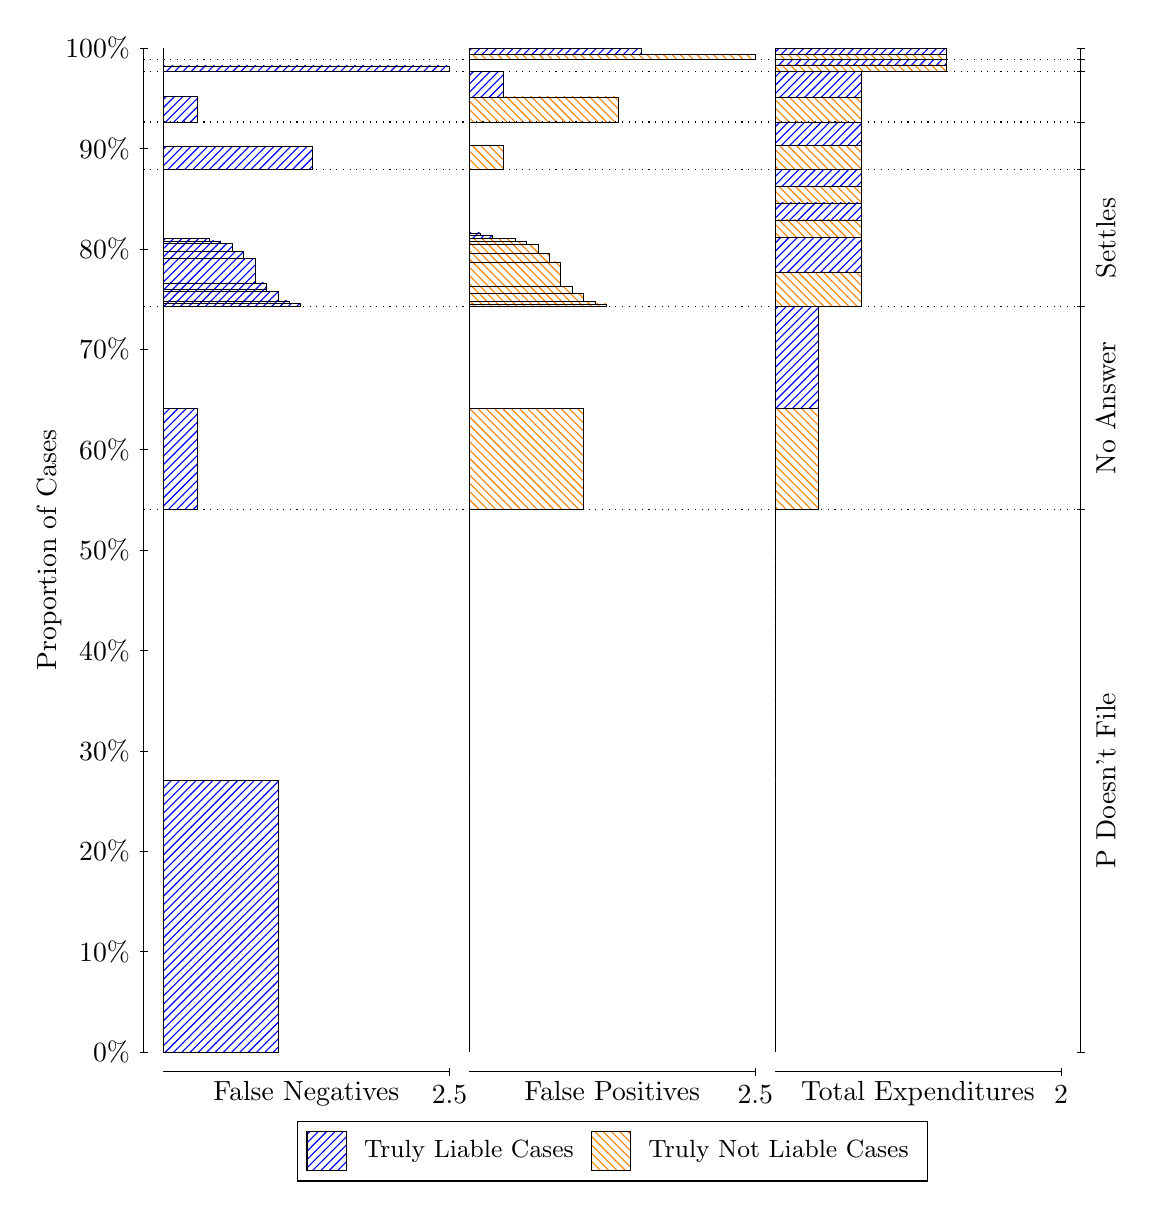
\begin{tikzpicture}
\draw[black, very thin] (1.5,1.75) -- (1.5,14.5);
\node[rotate=90, text=black, anchor=center] at (0.3, 8.125) {Proportion of Cases};
\draw[black, very thin] (1.45,1.75) -- (1.55,1.75);
\node[text=black, anchor=east] at (1.45, 1.75) {0\%};
\draw[black, very thin] (1.45,3.025) -- (1.55,3.025);
\node[text=black, anchor=east] at (1.45, 3.025) {10\%};
\draw[black, very thin] (1.45,4.3) -- (1.55,4.3);
\node[text=black, anchor=east] at (1.45, 4.3) {20\%};
\draw[black, very thin] (1.45,5.575) -- (1.55,5.575);
\node[text=black, anchor=east] at (1.45, 5.575) {30\%};
\draw[black, very thin] (1.45,6.85) -- (1.55,6.85);
\node[text=black, anchor=east] at (1.45, 6.85) {40\%};
\draw[black, very thin] (1.45,8.125) -- (1.55,8.125);
\node[text=black, anchor=east] at (1.45, 8.125) {50\%};
\draw[black, very thin] (1.45,9.4) -- (1.55,9.4);
\node[text=black, anchor=east] at (1.45, 9.4) {60\%};
\draw[black, very thin] (1.45,10.675) -- (1.55,10.675);
\node[text=black, anchor=east] at (1.45, 10.675) {70\%};
\draw[black, very thin] (1.45,11.95) -- (1.55,11.95);
\node[text=black, anchor=east] at (1.45, 11.95) {80\%};
\draw[black, very thin] (1.45,13.225) -- (1.55,13.225);
\node[text=black, anchor=east] at (1.45, 13.225) {90\%};
\draw[black, very thin] (1.45,14.5) -- (1.55,14.5);
\node[text=black, anchor=east] at (1.45, 14.5) {100\%};

\draw[black, very thin] (13.4,1.75) -- (13.4,14.5);
\draw[black, very thin] (13.35,1.75) -- (13.45,1.75);
\node[anchor=west] at (13.35, 1.75) {};
\draw[black, very thin] (13.35,8.6406) -- (13.45,8.6406);
\node[anchor=west] at (13.35, 8.6406) {};
\draw[black, very thin] (13.35,11.215) -- (13.45,11.215);
\node[anchor=west] at (13.35, 11.215) {};
\draw[black, very thin] (13.35,12.957) -- (13.45,12.957);
\node[anchor=west] at (13.35, 12.957) {};
\draw[black, very thin] (13.35,13.561) -- (13.45,13.561);
\node[anchor=west] at (13.35, 13.561) {};
\draw[black, very thin] (13.35,14.206) -- (13.45,14.206);
\node[anchor=west] at (13.35, 14.206) {};
\draw[black, very thin] (13.35,14.353) -- (13.45,14.353);
\node[anchor=west] at (13.35, 14.353) {};
\draw[black, very thin] (13.35,14.5) -- (13.45,14.5);
\node[anchor=west] at (13.35, 14.5) {};

\draw[black, very thin, pattern color=blue, pattern=north east lines] (1.75,1.75) rectangle (3.2033,5.1953);
\draw[black, very thin, pattern color=orange, pattern=north west lines] (1.75,5.1953) rectangle (1.75,8.6406);
\draw[black, very thin, pattern color=blue, pattern=north east lines] (1.75,8.6406) rectangle (2.186,9.928);
\draw[black, very thin, pattern color=orange, pattern=north west lines] (1.75,9.928) rectangle (1.75,11.215);
\draw[black, very thin, pattern color=blue, pattern=north east lines] (1.75,11.215) rectangle (3.494,11.254);
\draw[black, very thin, pattern color=blue, pattern=north east lines] (1.75,11.254) rectangle (3.3487,11.289);
\draw[black, very thin, pattern color=blue, pattern=north east lines] (1.75,11.289) rectangle (3.2033,11.41);
\draw[black, very thin, pattern color=blue, pattern=north east lines] (1.75,11.41) rectangle (3.058,11.432);
\draw[black, very thin, pattern color=blue, pattern=north east lines] (1.75,11.432) rectangle (3.058,11.518);
\draw[black, very thin, pattern color=blue, pattern=north east lines] (1.75,11.518) rectangle (2.9127,11.83);
\draw[black, very thin, pattern color=blue, pattern=north east lines] (1.75,11.83) rectangle (2.7673,11.921);
\draw[black, very thin, pattern color=blue, pattern=north east lines] (1.75,11.921) rectangle (2.622,12.021);
\draw[black, very thin, pattern color=blue, pattern=north east lines] (1.75,12.021) rectangle (2.4767,12.052);
\draw[black, very thin, pattern color=blue, pattern=north east lines] (1.75,12.052) rectangle (2.3313,12.087);
\draw[black, very thin, pattern color=orange, pattern=north west lines] (1.75,12.087) rectangle (1.75,12.957);
\draw[black, very thin, pattern color=blue, pattern=north east lines] (1.75,12.957) rectangle (3.6393,13.255);
\draw[black, very thin, pattern color=orange, pattern=north west lines] (1.75,13.255) rectangle (1.75,13.561);
\draw[black, very thin, pattern color=blue, pattern=north east lines] (1.75,13.561) rectangle (2.186,13.888);
\draw[black, very thin, pattern color=orange, pattern=north west lines] (1.75,13.888) rectangle (1.75,14.206);
\draw[black, very thin, pattern color=blue, pattern=north east lines] (1.75,14.206) rectangle (5.3833,14.274);
\draw[black, very thin, pattern color=orange, pattern=north west lines] (1.75,14.274) rectangle (1.75,14.353);
\draw[black, very thin, pattern color=orange, pattern=north west lines] (1.75,14.353) rectangle (1.75,14.421);
\draw[black, very thin, pattern color=blue, pattern=north east lines] (1.75,14.421) rectangle (1.75,14.5);
\draw[black, very thin, pattern color=orange, pattern=north west lines] (5.6333,1.75) rectangle (5.6333,5.1953);
\draw[black, very thin, pattern color=blue, pattern=north east lines] (5.6333,5.1953) rectangle (5.6333,8.6406);
\draw[black, very thin, pattern color=orange, pattern=north west lines] (5.6333,8.6406) rectangle (7.0867,9.928);
\draw[black, very thin, pattern color=blue, pattern=north east lines] (5.6333,9.928) rectangle (5.6333,11.215);
\draw[black, very thin, pattern color=orange, pattern=north west lines] (5.6333,11.215) rectangle (7.3773,11.25);
\draw[black, very thin, pattern color=orange, pattern=north west lines] (5.6333,11.25) rectangle (7.232,11.281);
\draw[black, very thin, pattern color=orange, pattern=north west lines] (5.6333,11.281) rectangle (7.0867,11.381);
\draw[black, very thin, pattern color=orange, pattern=north west lines] (5.6333,11.381) rectangle (6.9413,11.473);
\draw[black, very thin, pattern color=orange, pattern=north west lines] (5.6333,11.473) rectangle (6.796,11.784);
\draw[black, very thin, pattern color=orange, pattern=north west lines] (5.6333,11.784) rectangle (6.6507,11.891);
\draw[black, very thin, pattern color=orange, pattern=north west lines] (5.6333,11.891) rectangle (6.5053,12.011);
\draw[black, very thin, pattern color=orange, pattern=north west lines] (5.6333,12.011) rectangle (6.36,12.048);
\draw[black, very thin, pattern color=orange, pattern=north west lines] (5.6333,12.048) rectangle (6.2147,12.086);
\draw[black, very thin, pattern color=blue, pattern=north east lines] (5.6333,12.086) rectangle (5.924,12.12);
\draw[black, very thin, pattern color=blue, pattern=north east lines] (5.6333,12.12) rectangle (5.7787,12.152);
\draw[black, very thin, pattern color=blue, pattern=north east lines] (5.6333,12.152) rectangle (5.6333,12.957);
\draw[black, very thin, pattern color=orange, pattern=north west lines] (5.6333,12.957) rectangle (6.0693,13.263);
\draw[black, very thin, pattern color=blue, pattern=north east lines] (5.6333,13.263) rectangle (5.6333,13.561);
\draw[black, very thin, pattern color=orange, pattern=north west lines] (5.6333,13.561) rectangle (7.5227,13.879);
\draw[black, very thin, pattern color=blue, pattern=north east lines] (5.6333,13.879) rectangle (6.0693,14.206);
\draw[black, very thin, pattern color=orange, pattern=north west lines] (5.6333,14.206) rectangle (5.6333,14.286);
\draw[black, very thin, pattern color=blue, pattern=north east lines] (5.6333,14.286) rectangle (5.6333,14.353);
\draw[black, very thin, pattern color=orange, pattern=north west lines] (5.6333,14.353) rectangle (9.2667,14.421);
\draw[black, very thin, pattern color=blue, pattern=north east lines] (5.6333,14.421) rectangle (7.8133,14.5);
\draw[black, very thin, pattern color=orange, pattern=north west lines] (9.5167,1.75) rectangle (9.5167,5.1953);
\draw[black, very thin, pattern color=blue, pattern=north east lines] (9.5167,5.1953) rectangle (9.5167,8.6406);
\draw[black, very thin, pattern color=orange, pattern=north west lines] (9.5167,8.6406) rectangle (10.062,9.928);
\draw[black, very thin, pattern color=blue, pattern=north east lines] (9.5167,9.928) rectangle (10.062,11.215);
\draw[black, very thin, pattern color=orange, pattern=north west lines] (9.5167,11.215) rectangle (10.607,11.657);
\draw[black, very thin, pattern color=blue, pattern=north east lines] (9.5167,11.657) rectangle (10.607,12.1);
\draw[black, very thin, pattern color=orange, pattern=north west lines] (9.5167,12.1) rectangle (10.607,12.317);
\draw[black, very thin, pattern color=blue, pattern=north east lines] (9.5167,12.317) rectangle (10.607,12.534);
\draw[black, very thin, pattern color=orange, pattern=north west lines] (9.5167,12.534) rectangle (10.607,12.745);
\draw[black, very thin, pattern color=blue, pattern=north east lines] (9.5167,12.745) rectangle (10.607,12.957);
\draw[black, very thin, pattern color=orange, pattern=north west lines] (9.5167,12.957) rectangle (10.607,13.263);
\draw[black, very thin, pattern color=blue, pattern=north east lines] (9.5167,13.263) rectangle (10.607,13.561);
\draw[black, very thin, pattern color=orange, pattern=north west lines] (9.5167,13.561) rectangle (10.607,13.879);
\draw[black, very thin, pattern color=blue, pattern=north east lines] (9.5167,13.879) rectangle (10.607,14.206);
\draw[black, very thin, pattern color=orange, pattern=north west lines] (9.5167,14.206) rectangle (11.697,14.286);
\draw[black, very thin, pattern color=blue, pattern=north east lines] (9.5167,14.286) rectangle (11.697,14.353);
\draw[black, very thin, pattern color=orange, pattern=north west lines] (9.5167,14.353) rectangle (11.697,14.421);
\draw[black, very thin, pattern color=blue, pattern=north east lines] (9.5167,14.421) rectangle (11.697,14.5);
\draw[black, dotted] (1.5,8.6406) -- (13.4,8.6406);
\draw[black, dotted] (1.5,11.215) -- (13.4,11.215);
\draw[black, dotted] (1.5,12.957) -- (13.4,12.957);
\draw[black, dotted] (1.5,13.561) -- (13.4,13.561);
\draw[black, dotted] (1.5,14.206) -- (13.4,14.206);
\draw[black, dotted] (1.5,14.353) -- (13.4,14.353);
\draw[black, very thin] (1.75,1.5) -- (5.3833,1.5);
\node[text=black, anchor=north] at (3.5667, 1.5) {False Negatives};
\draw[black, very thin] (5.3833,1.45) -- (5.3833,1.55);
\node[text=black, anchor=north] at (5.3833, 1.45) {2.5};

\draw[black, very thin] (5.6333,1.5) -- (9.2667,1.5);
\node[text=black, anchor=north] at (7.45, 1.5) {False Positives};
\draw[black, very thin] (9.2667,1.45) -- (9.2667,1.55);
\node[text=black, anchor=north] at (9.2667, 1.45) {2.5};

\draw[black, very thin] (9.5167,1.5) -- (13.15,1.5);
\node[text=black, anchor=north] at (11.333, 1.5) {Total Expenditures};
\draw[black, very thin] (13.15,1.45) -- (13.15,1.55);
\node[text=black, anchor=north] at (13.15, 1.45) {2};

\node[text=black, centered, rotate=90] at (13.72, 5.1953) {P Doesn't File};
\node[text=black, centered, rotate=90] at (13.72, 9.928) {No Answer};
\node[text=black, centered, rotate=90] at (13.72, 12.086) {Settles};





\draw (7.449999999999999,1.5) node[draw=none] (baseCoordinate) {};
\begin{scope}[align=center]
        \matrix[scale=0.5, draw=black, below=0.5cm of baseCoordinate, nodes={draw}, column sep=0.1cm]{
            \node[rectangle, draw, minimum width=0.5cm, minimum height=0.5cm, pattern color=blue, pattern=north east lines] {}; &
            \node[draw=none, font=\small, text=black] (B) {Truly Liable Cases}; &
            \node[rectangle, draw, minimum width=0.5cm, minimum height=0.5cm, pattern color=orange, pattern=north west lines] {}; &
            \node[draw=none, font=\small, text=black] (B) {Truly Not Liable Cases}; \\
            };
\end{scope}

\end{tikzpicture}
\end{document}